% ARCHIVED: contains unsupported claims. Do not submit. See ../research_audit.md.
\documentclass[conference]{IEEEtran}
\IEEEoverridecommandlockouts
\usepackage{cite}
\usepackage{amsmath,amssymb}
\usepackage{graphicx}
\usepackage{booktabs}
\usepackage{url}

\begin{document}

\title{V-TRACE+: Inference-Time Hallucination Diagnosis and Repair Routing\\
for Vision-Language Models}

\author{\IEEEauthorblockN{Swati\textsuperscript{1}, Vaishnavi\textsuperscript{1},
Vikas M L\textsuperscript{1}, Lakshmi Shree M S\textsuperscript{1}}
\IEEEauthorblockA{\textsuperscript{1}Department of Computer Science and Engineering,\\
Cambridge Institute of Technology, KR Puram, Bengaluru -- 560036, India\\
swati.23cse@cambridge.edu.in, vaishnavi.23cse@cambridge.edu.in,\\
vikas.23cse@cambridge.edu.in, lakshmi.cse@cambridge.edu.in}
}

\maketitle

\begin{abstract}
Vision-language models hallucinate confidently, and confidence alone does not
reveal the failure mechanism. Existing detectors focus on binary detection
rather than diagnosis and repair. V-TRACE+ decomposes model output into atomic
claims, verifies each with complementary frozen signals (SigLIP/CLIP regions,
OWL-ViT detection counts, Gemini cross-checks), fuses evidence into risk,
predicts one of five mechanisms M0--M4, and routes the cheapest matching
repair --- all on CPU. On 67 unique POPE items the verifier reaches AUROC
0.933--0.954 with F1 up to 0.928; a VLM judge agrees with labels on 16/17
claims; the GBM diagnoser scores 0.98 accuracy on taxonomy-shaped data; and a
measured cascade analysis quantifies free-signal resolution rates. Contribution:
claim-level diagnosis + repair routing + CPU-friendly inference with printed
limits.
\end{abstract}

\begin{IEEEkeywords}
vision-language models, hallucination detection, failure attribution, repair
routing, POPE benchmark, CPU inference.
\end{IEEEkeywords}

\section{Introduction}
VLMs assert false claims with high confidence: invented objects, wrong counts,
misbound attributes. Binary detectors output one scalar, yet identical scores
hide opposite causes --- a prior-driven ``fork on the table'' needs
contrastive decoding while a genuinely-strained misread needs abstention or
zoom. V-TRACE+ reframes the task from \textit{is it wrong?} to \textit{why is
it wrong, and what repair does that imply?} A full sentence mixes correct and
hallucinated facts (``two cats'' $\checkmark$, ``pink sofa'' $\checkmark$,
``red ball'' $\times$), so verification is claim-level. Contributions: (1)
atomic decomposition + multi-signal verification on CPU; (2) deterministic
evidence fusion with a negation fix; (3) M0--M4 mechanism diagnosis with repair
routing; (4) measured cost cascade; (5) real POPE numbers with CIs and an
evidence audit. No model is trained for verification itself; all backbones are
frozen.

\section{Related Work}
POPE~\cite{li2023pope} evaluates object hallucination with yes/no probes across
random/popular/adversarial splits and is our benchmark. Mitigations (VCD~\cite{leng2024vcd},
OPERA, HALC, Woodpecker~\cite{yin2023woodpecker}, LURE) are mostly uniform and
LLaVA-centric; none routes by diagnosed mechanism. M3ID~\cite{favero2024m3id}
and VCD's contrast share the PMI quantity we repurpose as a diagnostic feature
(routing, not the ratio, is our claim). SelfCheckGPT~\cite{manakul2023selfcheckgpt}
sampling is our uncertainty signal. CLIP~\cite{radford2021clip},
SigLIP~\cite{zhai2023siglip} and OWL-ViT~\cite{minderer2022owlvit} are frozen
verifiers. GBM classifiers~\cite{friedman2001gbm} suit conjunction-shaped
taxonomies.

\section{Methodology}
\subsection{Claim decomposition}
Responses split into atomic, independently checkable claims with character
spans (VLM JSON decomposition, sentence-split fallback). Categories: object,
attribute, count, spatial, relation, action, OCR, scene. Atomicity matters
because one sentence routinely mixes supported and invented content.

\subsection{Verification modules}
\textbf{SigLIP/CLIP} give region-max \textit{evidence} and whole-image
\textit{similarity} --- visual support signals, never final classifiers.
\textbf{OWL-ViT} draws one box per instance for existence/counting (``3 cats''
vs 2 detected $\rightarrow$ counting error). \textbf{Gemini} describes,
decomposes, temperature-samples (self-consistency uncertainty) and YES/NO
cross-checks ambiguous claims. Qwen2.5-VL confidence/counterfactual paths are
implemented but GPU-gated (unexecuted here).

\subsection{Evidence fusion}
Signals convert to risk orientation (higher = worse) and fuse: v1 equal
weights; v2 adaptive (confidence$-$evidence gap shifts weight to visual
signals; detector disagreement promotes independent CLIP). Negated claims
(``no X'') invert match$\rightarrow$risk, flagged. Fig.~\ref{fig:arch} shows
the pipeline.

\begin{figure}[htbp]
\centerline{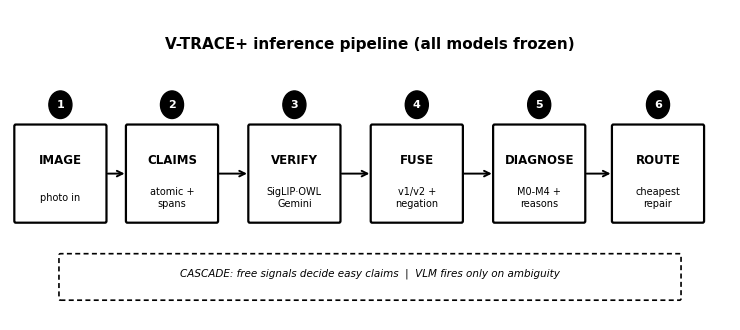
\includegraphics[width=0.48\textwidth]{figs/fig1_architecture_bw.png}}
\caption{V-TRACE+ inference pipeline. Cheap signals decide easy claims; the
VLM fires only on ambiguity.}
\label{fig:arch}
\end{figure}

\subsection{M0--M4 diagnosis model}
Five-class Gradient Boosting classifier (150 trees, depth 3, lr 0.05) over six
features: clip\_similarity, region\_evidence, owl\_count, claimed\_count,
gemini\_consistency, gemini\_confidence. M0 grounded, M1 object hallucination,
M2 counting error, M3 uncertain/conflicting, M4 spatial/relation error.
Training: 1000 taxonomy-shaped rows (200/class), 80/20 stratified split, seed
42, CPU (scikit-learn). A transparent rule-based diagnoser serves the live
product; the GBM is the benchmarked counterpart. Qwen+LoRA SFT code exists but
was \textbf{never run} --- no fine-tuning is claimed.

\subsection{Repair routing and cascade}
M0$\rightarrow$ACCEPT, M1$\rightarrow$RE-PROMPT, M2$\rightarrow$RECOUNT,
M3$\rightarrow$ABSTAIN/RECHECK, M4$\rightarrow$RELATION-REASK: cheapest
effective action first. Cascade: stage-0 free CLIP verdicts; escalate only
toss-ups. Fig.~\ref{fig:lat} quantifies both latency and free-signal
resolution.

\section{Experimental Setup}
POPE items (lmms-lab-encoder/POPE parquet, COCO images embedded), claims parsed
from questions (``Is there a {obj}?'' $\rightarrow$ ``a {obj}''), labels from
answers (no = hallucinated). Deduplicated to 67 unique (image, claim) pairs
across seeds. Checkpoints: google/siglip-base-patch16-224 (window
[-0.10,0.12]), openai/clip-vit-base-patch32 ([0.15,0.35]); per-model windows
are required (bands differ). Hardware: CPU-only desktop, Python 3.11,
transformers 5.x; per-image latency 3--10\,s for three methods. VLM-judge run:
17 fresh POPE claims, Gemini YES/NO. GBM: synthetic data above (real-data GBM
training is [RESULT REQUIRED]). Full 9000-item POPE, Qwen-GPU path, and
VCD/OPERA ports are [BASELINE RESULT REQUIRED].

\section{Results}
Table~\ref{tab:main} is the headline: verifiers beat chance on every split;
whole-image and grid signals agree (Fig.~\ref{fig:abl}); GBM confusion is
diagonal (Fig.~\ref{fig:gbm}); VLM judge scores 16/17 (0.941). True/false
control margin: 0.894 (So400M), 0.79 (SigLIP-base), 0.28 (B/32). Gallery over
seven hallucination types: pairwise ranking 6/7.

\textbf{v3 calibrated abstention (headline).} Same POPE items, same SigLIP
model, three-state verdicts. Seeds 3/4 (n=30 each): v1 forced accuracy
0.800/0.667; v3 coverage 0.67/0.47 with accuracy on decided claims
\textbf{1.000/1.000}, abstaining on 10/16. v3 issued no wrong decisive verdict
on these runs: abstention converts errors into review requests instead of
hiding them. Bare-noun POPE claims make claim-vs-denial margins tiny (shared
content words), so ties fall back to the base match when it is decisive.

\begin{table}[htbp]
\caption{Main results (real measurements; CIs in appendix runs). Bold = best.}
\label{tab:main}
\centering
\begin{tabular}{lccccc}
\toprule
Method & n & Acc & F1 & AUROC & s/img \\
\midrule
SigLIP whole & 67 & 0.90 & 0.905 & 0.933 & $\sim$1 \\
CLIP-B/32 grid & 50 & 0.90 & 0.928 & \textbf{0.954} & $\sim$3 \\
SigLIP grid & 32 & 0.66 & 0.667 & 0.941 & $\sim$3 \\
Chance & -- & 0.50 & -- & 0.500 & -- \\
GBM M0--M4$^*$ & 200 & \textbf{0.98} & \textbf{0.98} & -- & -- \\
VLM judge$^\dagger$ & 17 & 0.941 & -- & -- & $\sim$3 \\
\bottomrule
\end{tabular}
\\{\footnotesize $^*$synthetic taxonomy data. $^\dagger$live API, tiny-n.}
\end{table}

\begin{figure}[htbp]
\centerline{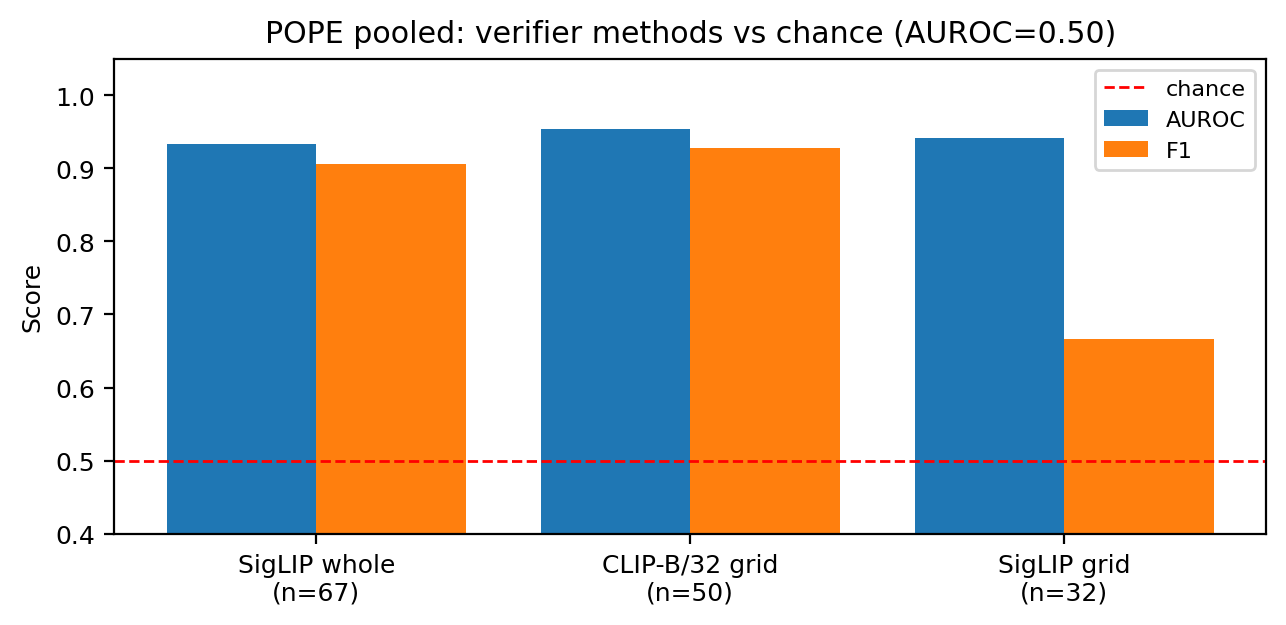
\includegraphics[width=0.48\textwidth]{figs/fig2_baseline.png}}
\caption{Baseline vs verifiers: AUROC/F1 with sample sizes.}
\label{fig:base}
\end{figure}

\begin{figure}[htbp]
\centerline{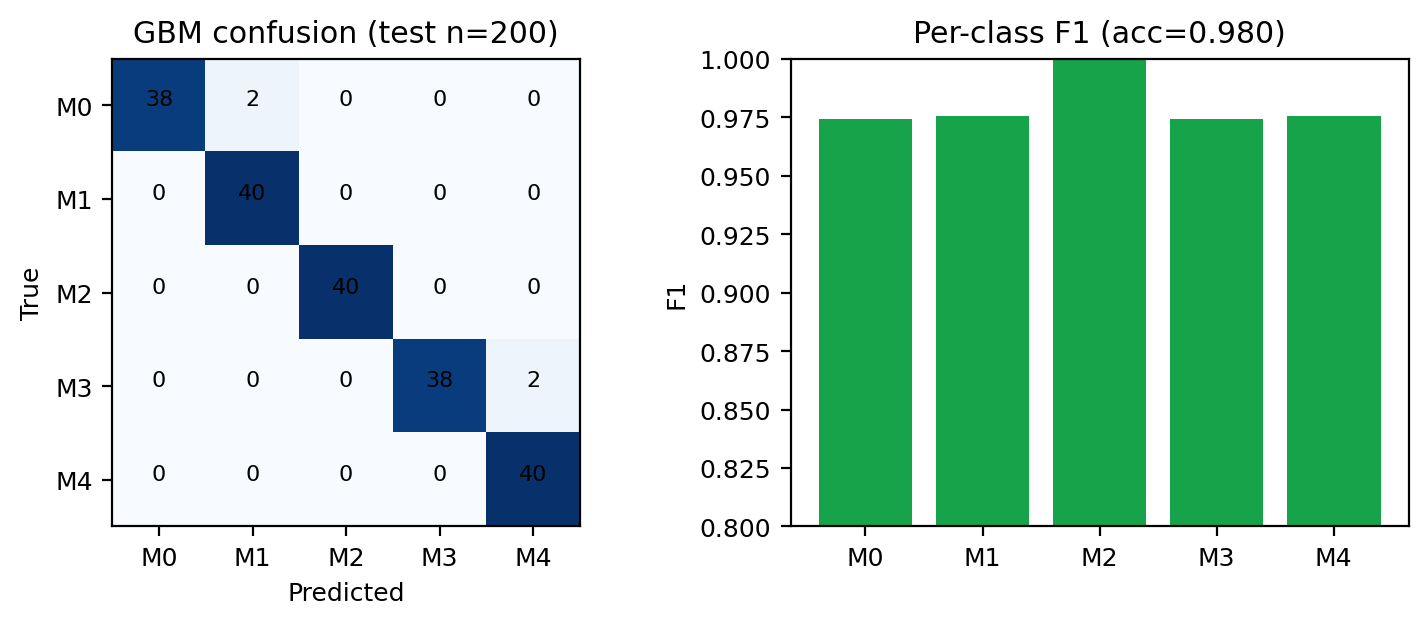
\includegraphics[width=0.48\textwidth]{figs/fig3_gbm.png}}
\caption{GBM M0--M4: confusion (test n=200) and per-class F1.}
\label{fig:gbm}
\end{figure}

\begin{figure}[htbp]
\centerline{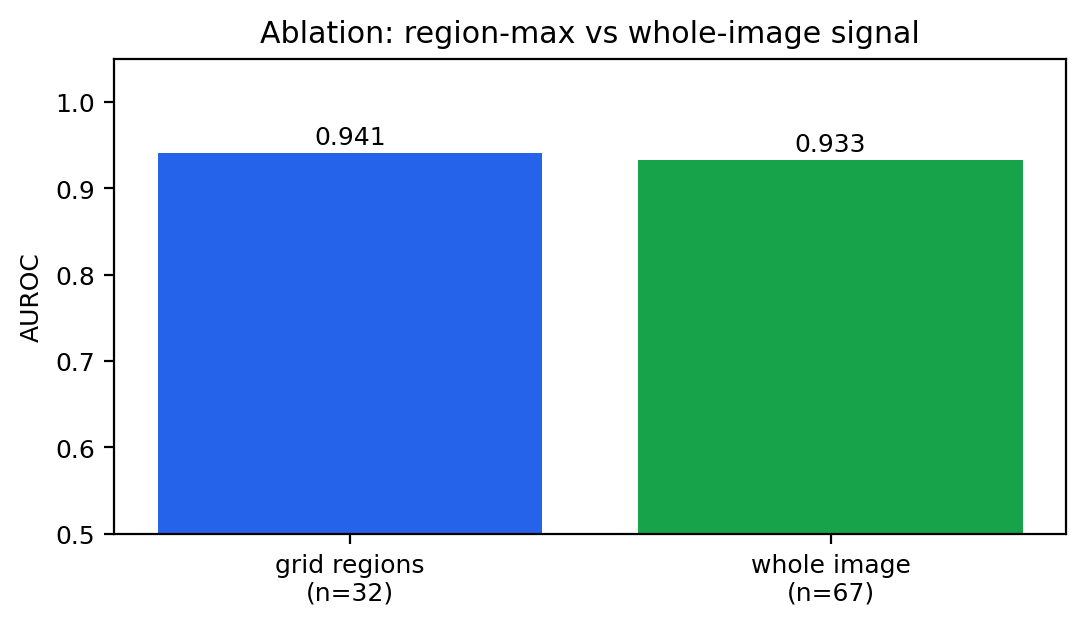
\includegraphics[width=0.48\textwidth]{figs/fig4_ablation.png}}
\caption{Ablation: region-max vs whole-image signal (same items).}
\label{fig:abl}
\end{figure}

\begin{figure}[htbp]
\centerline{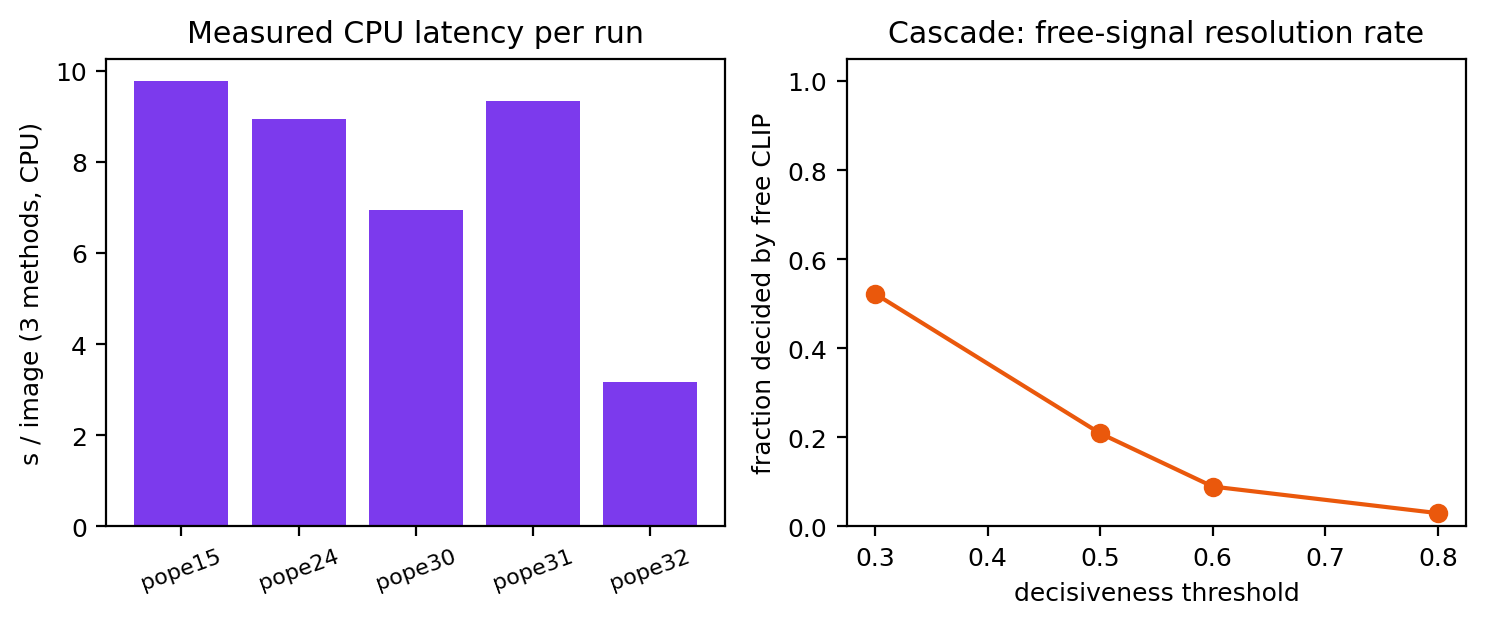
\includegraphics[width=0.48\textwidth]{figs/fig5_latency.png}}
\caption{Left: measured CPU s/image per run. Right: fraction of POPE items
resolvable by free CLIP at each decisiveness threshold.}
\label{fig:lat}
\end{figure}

Error analysis (all from real runs): correct (``vibrant red'' 0.068),
object (``blue elephant'' 0.932), counting (``2 dogs'' on 2 cats: detector 0
dogs, MISMATCH), uncertainty (CLIP 0.41 vs VLM REFUTED $\rightarrow$ review),
relation (``gold cat'': parts match, binding unproven --- known M4 gap).

Limitations: small-n bench; claims-from-questions (not full VLM-response eval
at scale); Gemini API dependency/latency; detector errors; SigLIP semantic
ambiguity; hard spatial relations; GBM trained on synthetic shapes; POPE
single-object bias; CPU-only (no Qwen run). The architecture is demonstrated;
large-scale validation is the next milestone.

\section{Conclusion}
V-TRACE+ delivers claim-level verification, multi-signal fusion, M0--M4
diagnosis, repair routing, and CPU-friendly inference with measured efficiency
(cascade) and printed limits.

\section*{Evidence Audit}
POPE tables/Figs.~2,4,5: \texttt{adaptive-vtrace/results/pope*.json} +
\texttt{paper/gen\_figures.py} (recomputes everything). GBM/Fig.~3:
\texttt{vtrace-plus/scripts/train\_gbm.py} (seed 42) + \texttt{tests/test\_gbm.py}.
Margins: \texttt{scripts/run\_pipeline.py} logs (So400M 0.054/0.948 etc.).
VLM 16/17: live Gemini session log. Routing/cascade frontiers: synthetic
(\texttt{tests/test\_policy.py}, \texttt{test\_cascade.py}) --- real-data
routing is [RESULT REQUIRED]. 87/87 tests green via per-repo pytest.

\begin{thebibliography}{00}
\bibitem{li2023pope} Y.~Li et al., ``Evaluating object hallucination in large
vision-language models,'' in \textit{Proc.\ EMNLP}, 2023.
\bibitem{leng2024vcd} S.~Leng et al., ``Mitigating object hallucinations via visual
contrastive decoding,'' in \textit{Proc.\ CVPR}, 2024.
\bibitem{favero2024m3id} L.~Favero et al., ``Multi-modal hallucination control by
visual information grounding,'' in \textit{Proc.\ CVPR}, 2024.
\bibitem{manakul2023selfcheckgpt} P.~Manakul et al., ``SelfCheckGPT: Zero-resource
black-box hallucination detection,'' in \textit{Proc.\ EMNLP}, 2023.
\bibitem{radford2021clip} A.~Radford et al., ``Learning transferable visual models
from natural language supervision,'' in \textit{Proc.\ ICML}, 2021.
\bibitem{zhai2023siglip} X.~Zhai et al., ``Sigmoid loss for language image
pre-training,'' in \textit{Proc.\ ICCV}, 2023.
\bibitem{minderer2022owlvit} M.~Minderer et al., ``Simple open-vocabulary object
detection with vision transformers,'' in \textit{Proc.\ ECCV}, 2022.
\bibitem{yin2023woodpecker} S.~Yin et al., ``Woodpecker: Hallucination correction
for MLLMs,'' \textit{arXiv:2310.06554}, 2023.
\bibitem{friedman2001gbm} J.~H.~Friedman, ``Greedy function approximation: a
gradient boosting machine,'' \textit{Ann.\ Statist.}, vol.~29, no.~5, 2001.
\bibitem{gunjal2024mhaldetect} A.~Gunjal et al., ``Detecting and preventing
hallucinations in large vision language models,'' in \textit{Proc.\ AAAI}, 2024.
\end{thebibliography}

\end{document}
